% Schema del modello definito in 04_blocks.py, nella variante finale
% (3 blocchi + residui e proiezioni + feed forward largo), disegnato nello
% stile della Figura 1 di "Attention Is All You Need".
%
% Rispetto allo schema del file 03 le novita' sono tre: il Block, che raggruppa
% comunicazione e computazione e viene ripetuto 3 volte; il flusso residuo, cioe'
% le somme che bypassano ogni sotto-livello; e le proiezioni che riportano nel
% flusso residuo l'uscita di ogni sotto-livello.
%
% Compilare con:
%     pdflatex 04_out_architecture.tex
%     tectonic 04_out_architecture.tex

\documentclass[tikz,border=8pt]{standalone}

\usepackage[T1]{fontenc}
\usepackage{lmodern}
\usetikzlibrary{positioning,fit,calc,arrows.meta,backgrounds}

% i colori pastello della figura originale
\definecolor{cEmb}{RGB}{248,214,216}
\definecolor{cAtt}{RGB}{252,224,187}
\definecolor{cFF}{RGB}{200,225,245}
\definecolor{cLin}{RGB}{216,214,238}
\definecolor{cSM}{RGB}{205,235,205}
\definecolor{cBlk}{RGB}{240,240,240}

\begin{document}
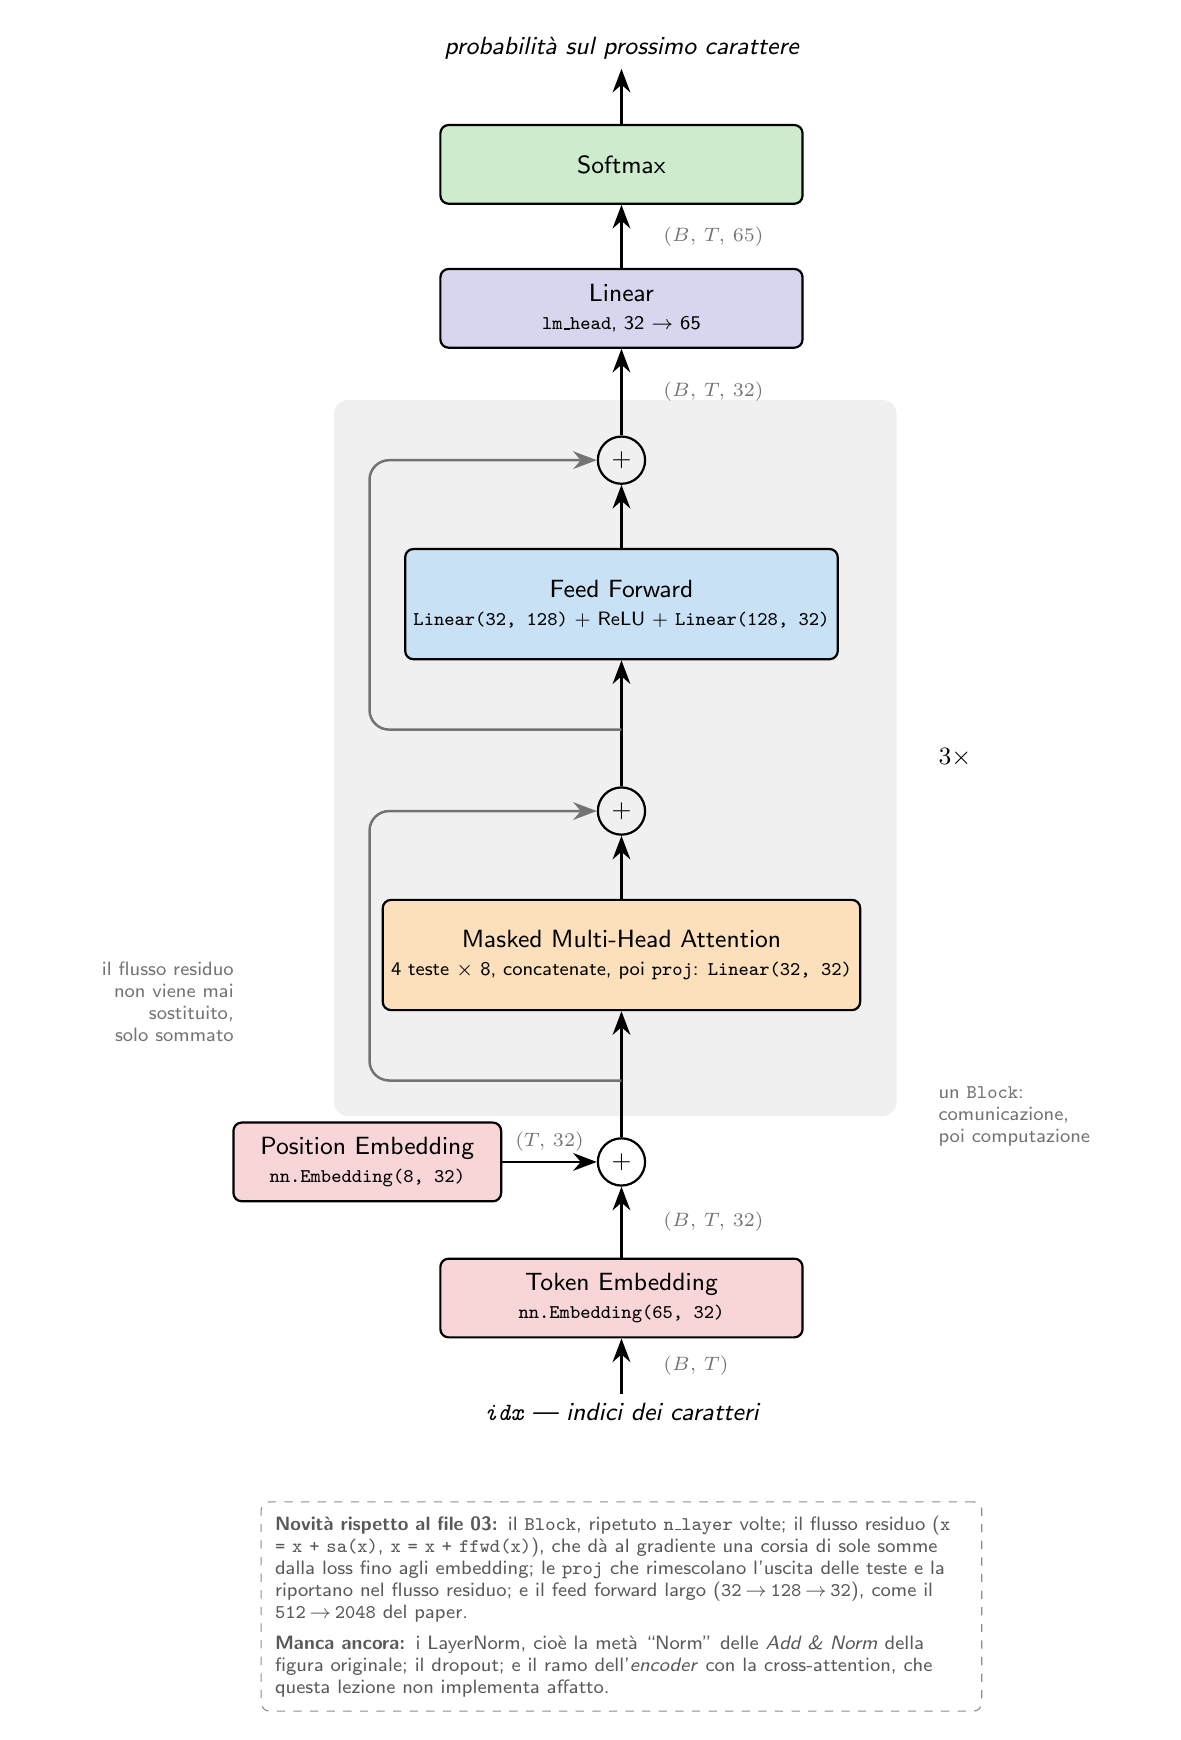
\begin{tikzpicture}[
  font=\sffamily\small,
  box/.style   = {draw, thick, rounded corners=3pt, align=center,
                  minimum width=46mm, minimum height=10mm, inner sep=3pt},
  sum/.style   = {draw, thick, circle, minimum size=6mm, inner sep=0pt},
  io/.style    = {align=center, font=\sffamily\small\itshape},
  flow/.style  = {-{Stealth[length=3mm]}, line width=0.9pt},
  res/.style   = {-{Stealth[length=3mm]}, line width=0.9pt, black!55},
  shp/.style   = {font=\sffamily\scriptsize, text=black!55,
                  anchor=west, xshift=4mm},
  tag/.style   = {font=\sffamily\scriptsize, text=black!55},
  note/.style  = {draw=black!45, dashed, rounded corners=3pt, align=left,
                  font=\sffamily\scriptsize, text=black!65, inner sep=5pt}
]

% ---------------------------------------------------------------- il flusso --
\node[io]                                   (inp) {\texttt{idx} \textemdash{} indici dei caratteri};
\node[box, fill=cEmb, above=7mm of inp]     (tok) {Token Embedding\\[-1pt]{\scriptsize\texttt{nn.Embedding(65, 32)}}};
\node[sum, above=9mm of tok]                (add0) {$+$};
\node[box, fill=cEmb, left=12mm of add0,
      minimum width=34mm]                   (pos) {Position Embedding\\[-1pt]{\scriptsize\texttt{nn.Embedding(8, 32)}}};

% --- il Block: comunicazione, poi computazione, ognuna dentro un residuo ---
\node[box, fill=cAtt, above=16mm of add0,
      minimum height=14mm]                  (mha) {Masked Multi-Head Attention\\[-1pt]{\scriptsize 4 teste $\times$ 8, concatenate, poi \texttt{proj}: \texttt{Linear(32, 32)}}};
\node[sum, above=8mm of mha]                (add1) {$+$};
\node[box, fill=cFF, above=16mm of add1,
      minimum height=14mm]                  (ff)  {Feed Forward\\[-1pt]{\scriptsize\texttt{Linear(32, 128)} + ReLU + \texttt{Linear(128, 32)}}};
\node[sum, above=8mm of ff]                 (add2) {$+$};

\node[box, fill=cLin, above=11mm of add2]   (lm)  {Linear\\[-1pt]{\scriptsize\texttt{lm\_head}, 32 $\rightarrow$ 65}};
\node[box, fill=cSM, above=8mm of lm]       (sm)  {Softmax};
\node[io, above=7mm of sm]                  (outp) {probabilit\`a sul prossimo carattere};

% ------------------------------------------------------------------- archi --
\draw[flow] (inp) -- (tok) node[shp, midway] {$(B,\,T)$};
\draw[flow] (tok) -- (add0) node[shp, midway] {$(B,\,T,\,32)$};
\draw[flow] (pos) -- (add0) node[tag, midway, above] {$(T,\,32)$};

% il flusso residuo: da s1 ci scostiamo, calcoliamo la self-attention, e
% rientriamo sommando in add1. idem da s2 per il feed forward. il giro passa
% a sinistra dei box (r1, r2), non sopra
\coordinate (s1) at ($(add0.north)!0.45!(mha.south)$);
\coordinate (s2) at ($(add1.north)!0.45!(ff.south)$);
\coordinate (r1) at ([xshift=-32mm]s1);
\coordinate (r2) at ([xshift=-32mm]s2);

\draw[line width=0.9pt] (add0) -- (s1);
\draw[flow] (s1) -- (mha);
\draw[res, rounded corners=2.5mm] (s1) -- (r1) |- (add1.west);

\draw[line width=0.9pt] (add1) -- (s2);
\draw[flow] (s2) -- (ff);
\draw[res, rounded corners=2.5mm] (s2) -- (r2) |- (add2.west);

\draw[flow] (mha) -- (add1);
\draw[flow] (ff)  -- (add2);

\draw[flow] (add2) -- (lm) node[shp, midway] {$(B,\,T,\,32)$};
\draw[flow] (lm)   -- (sm) node[shp, midway] {$(B,\,T,\,65)$};
\draw[flow] (sm)   -- (outp);

% ------------------------------------------------- il Block, ripetuto 3 volte --
\begin{scope}[on background layer]
  \node[fill=cBlk, rounded corners=5pt, fit=(mha)(add1)(ff)(add2)(r1)(r2),
        inner sep=4.5mm] (blk) {};
\end{scope}
\node[font=\sffamily\small, right=4mm of blk] {$3\times$};
\node[tag, above right=0mm and 4mm of blk.south east, anchor=west,
      text width=26mm] {un \texttt{Block}:\\comunicazione,\\poi computazione};

% ------------------------------------------------------------- annotazioni --
\node[tag, anchor=east, text width=25mm, align=right]
  at ([xshift=-16mm, yshift=10mm]r1) {il flusso residuo\\non viene mai\\sostituito,\\solo sommato};

% -------------------------------------------------------------- cosa manca --
\node[note, below=9mm of inp, text width=88mm] (nota) {%
  \textbf{Novit\`a rispetto al file 03:} il \texttt{Block}, ripetuto
  \texttt{n\_layer} volte; il flusso residuo (\texttt{x = x + sa(x)},
  \texttt{x = x + ffwd(x)}), che d\`a al gradiente una corsia di sole somme
  dalla loss fino agli embedding; le \texttt{proj} che rimescolano l'uscita
  delle teste e la riportano nel flusso residuo; e il feed forward largo
  (\texttt{32\,$\to$\,128\,$\to$\,32}), come il \texttt{512\,$\to$\,2048}
  del paper.\\[3pt]
  \textbf{Manca ancora:} i LayerNorm, cio\`e la met\`a ``Norm'' delle
  \emph{Add \& Norm} della figura originale; il dropout; e il ramo
  dell'\emph{encoder} con la cross-attention, che questa lezione non
  implementa affatto.};

\end{tikzpicture}
\end{document}
